\newcommand*{\DocType}{scrartcl}
%\newcommand*{\DocType}{article}
\newcommand*\ClassList{scrartcl,article}

\documentclass[\DocType, abstract=on, paper=a4, fontsize=11pt]{generalclass}

% Packages
\usepackage[a4paper]{geometry}
\usepackage[english]{babel}
\usepackage[utf8]{inputenc}
\usepackage[automark]{scrpage2}
\usepackage{xargs} % Use more than one optional parameter in a new commands
\usepackage[pdftex,dvipsnames]{xcolor}  % Coloured text etc.
\usepackage{graphicx} % Images etc.
\usepackage{amssymb}
\usepackage{amsmath}
\usepackage{mathtools} % e.g ":=" 
\usepackage[super]{nth} % use superscripts for 1st, 2nd, 3rd
\usepackage[numbers, square]{natbib} % citeauthor, citet
\usepackage{physics} % norm
\usepackage{enumitem} % changing enumeration styles
\usepackage{gensymb} % degree
\usepackage{booktabs} % nice table separators
\usepackage{tabularx} % better tables, X column
\usepackage{caption} % change style of figure 
\usepackage{subcaption} % subfigures
\usepackage{tikz} % for pgfplots
\usepackage{pgfplots} % plotting data
\usepackage[section]{placeins} % place figures in the sections they appear in
\usetikzlibrary{pgfplots.groupplots}


\captionsetup{justification=raggedright, format=plain, font=small,labelfont=bf}


\usepackage{xr-hyper}  
\usepackage[hidelinks, pagebackref,pdftex]{hyperref}

\usepackage[colorinlistoftodos,prependcaption,textsize=tiny]{todonotes}

\IfClass{article}{ % Optimize for screen
	\geometry{papersize={200mm,200mm},margin=5mm} 
}


\newcommandx{\unsure}[2][1=]{\todo[linecolor=orange,backgroundcolor=orange!25,bordercolor=orange,#1]{#2}}
\newcommandx{\Todo}[2][1=]{\todo[linecolor=yellow,backgroundcolor=yellow!25,bordercolor=yellow,#1]{#2}}
\newcommandx{\info}[2][1=]{\todo[linecolor=green,backgroundcolor=green!25,bordercolor=green,#1]{#2}}

\newcolumntype{Y}{>{\centering\arraybackslash}X} % centered equidistant columns

\setenumerate{label=(\arabic*),itemsep=0mm} % enumerate labeling and line distance
\renewcommand{\baselinestretch}{1.1} % line distance
\allowdisplaybreaks % Make big equations breakable


\pagenumbering{gobble}

\begin{document}
	\newgeometry{bottom=4cm}
\begin{titlepage}
	\centering
	
	\large{\textbf{Bachelor's Thesis}}
	\vspace{0.4cm}
	
	\huge{\textbf{Effects of Pose Normalization on Weakly Supervised 3D Human Pose Estimation}}\par
	
	\vspace{1cm}
	\Large{Nikolas Klug}
	
	\vspace{1cm}
	\Large{September 2019}
	
	\vspace{\fill}
	
\includegraphics[scale=0.5]{figures/Uni_Aug_Logo_FAI_RGB.png}
	\vspace{5mm}
	
	University of Augsburg
	
	Department of Computer Science
	
	Multimedia Computing and Computer Vision Lab
\end{titlepage}

\normalfont
\restoregeometry
\pagebreak


	
	{
	\newgeometry{bottom=2cm}
	\vspace*{19.5cm}
	
	\Large{
	\def\arraystretch{1.2}
	\begin{tabular}{l l}
	
		\textbf{Reviewer:} & Prof. Dr. Rainer Lienhart\\
		\textbf{Second Reviewer:} & Prof. Dr. Elisabeth André\\
		\textbf{Advisor:} & Moritz Einfalt
	
	\end{tabular}
	}\par
	
	\def\arraystretch{1}
}
\restoregeometry
\pagebreak
	
	\begin{polyabstract}{Abstract}
	With well-performing 2D human pose estimators evolving over the last years, recent work focuses on inferring 3D poses from 2D poses.
	During the ECCV 2018 Workshops, Drover et al. presented such a 2D to 3D pose estimator in their work "Can 3D Pose be Learned from 2D Projections Alone?".
	Using a Generative Adversarial Network, their system is able to achieve state of the art results.
	On top of that, its main feature is that no 3D ground truth poses are required for training, which makes it especially attractive in applications where no ground truth data is available.
	
	In their proposed system, Drover et al. require the 2D input poses to be normalized in scale and position.
	The goal of this thesis is to analyze the effects of this normalization on the qualitative performance of the 3D pose estimation in that system.
	For this, baseline results for synthetically generated poses are established in a first step.
	Subsequently, the effects of normalization in position and scale are analyzed.
	Both the theoretical findings and the conducted experiments show that the normalization indeed negatively influences the measurable error.
	Since especially the normalization in position accounts for a significant increase in error, the system is modified to compensate for this.
	
	In addition to the analysis of the effects of normalization, an alternative loss function is proposed.
	It leverages high-level knowledge about the structure of human poses to produce improved results.
	With this new loss function, the error can be reduced by more than $7\%$. 
	
\end{polyabstract}

\pagebreak
\selectlanguage{german}
\begin{polyabstract}{Zusammenfassung}
	Da in den letzten Jahren leistungsstarke 2D Posenerkennungssysteme entwickelt wurden, liegt der Fokus der jüngsten Forschung darauf, aus diesen 2D Posen 3D Posen zu generieren.
	Während den ECCV 2018 Workshops haben Drover et al. in ihrer Arbeit \glqq Can 3D Pose be Learned from 2D Projections Alone?\grqq (in etwa \glqq Können 3D Posen ausschließlich von 2D Projektionen erlernt werden?\grqq) ein solches System vorgestellt, das für menschliche 2D Posen die dazugehörigen 3D Posen generiert.
	Mit Hilfe eines Generative Adversarial Networks gelingt es diesem System Ergebnisse zu erzielen, die dem aktuellen Stand der Technik entsprechen.
	Darüberhinaus bietet das System den großen Vorteil, dass für das Training keine 3D Grundwahrheitsposen benötigt werden.
	Dies macht das System besonders für Anwendungen attraktiv, in denen keine Grundwahrheitsdaten vorhanden sind.
	
	In dem von Drover et al. vorgestellten System müssen die 2D Eingabeposen in Größe und Position normalisiert sein.
	Das Ziel dieser Arbeit ist es, die Effekte dieser Normalisierung auf die qualitative Leistungsfähigkeit der 3D-Posengenerierung zu analysieren.
	Dafür werden als Erstes Ausgangsresultate für synthetisch generierte Posen ermittelt.
	Anschließend werden die Effekte der Größen- und Positionsnormalisierung analysiert.
	Sowohl die theoretische Untersuchung als auch die durchgeführten Experimente zeigen, dass die Normalisierung den messbaren Fehler negativ beeinflusst.
	Da insbesondere die Größennormalisierung für einen deutlichen Anstieg des Fehlers verantwortlich ist, wird das System so modifiziert, dass der zusätzliche Fehler kompensiert wird.
	
	Zusätzlich zur Analyse der Effekte der Posennormalisierung wird eine alternative Fehlerfunktion vorgestellt.
	Diese verwendet allgemeines Wissen über die Struktur menschlicher Posen, um verbesserte Ergebnisse zu erzielen.
	Mit der neuen Fehlerfunktion kann der Fehler um mehr als $7\%$ reduziert werden. 
\end{polyabstract}

\selectlanguage{english}
	\pagebreak
	
	\tableofcontents
	\pagebreak
	
	\pagenumbering{arabic}

	\Todo[inline]{Beim Korrekturlesen darauf achten ob Sachen benutzt werden, die vorher nicht erläutert wurden. Außerdem:
		Werden die Zusammenhänge überall klar?
		Wird die Motivation, bestimmte Dinge zu tun/ zu analysieren klar?
	}
	\section{Introduction}

Human pose estimation has gained a lot of attention in the last years.
With the emergence of models that are able to accurately estimate poses in real-time from RGB images only, pose tracking has now become more accessible than ever.
Systems like DeepCut \cite{pishchulin16}, the Stacked Hourglass architecture \cite{newell16} and most recently OpenPose \cite{cao18} are able to infer two dimensional (2D) human poses from RGB images with high precision.
With those well-performing 2D pose estimators, the next logical step is to estimate poses in three dimensions (3D).
For this, some end-to-end frameworks have been proposed, which estimate the 3D poses directly from RGB images \cite{pavlakos17, park16, mehta17, mehta17_2}.
Another approach is to split the task of 3D pose estimation into two subtasks \cite{drover18, martinez17, moreno-noguer16}:
2D pose estimation from RGB images and subsequent 3D pose estimation from the 2D poses.
This two-step pipeline benefits from the fact that the existing 2D pose estimators can be used for the first part, which means that 3D pose estimation is reduced to the second subtask, that is, the to 2D to 3D lifting.

Human pose estimation has been successfully applied in multiple areas.
In the medical field human pose estimation can help in detecting any movement related disorders.
\citet{aroeira16} use pose estimation to detect scoliosis in adolescents through the analysis of their postures.
In another work, \citet{khan18} use poses to monitor Vojta therapy, a form of therapy treating motor disabilities originating from neurological disorders.
Pose estimation is also necessary in future personal care robots that may be used in the context of assisted living \cite{richter15}.
Apart from applications in the medical field, an obvious application of human pose estimation is replacing the systems that are currently used for the task.
Concretely, those are Motion Capture (MoCap) systems used e.g. for animations and visualizations and RGBD cameras like Microsoft Kinect.
Not only are those systems expensive, but can also not be used in all environments (especially MoCap).
Here, pose estimation from RGB images only can provide a cheaper, more easily accessible alternative.
Human pose estimation can also be of help in the performance analysis of athletes in sports \cite{einfalt18, zecha19}.
Further applications include monitoring human behavior in surveillance scenarios, in working environments or elsewhere.

\subsection{"Can 3D Pose be Learned from 2D Projections Alone?"}

As explained above, recent work in the field of 3D pose estimation focuses on lifting 2D poses into three dimensions. 
In the paper "Can 3D Pose be Learned from 2D Projections Alone?", \citet{drover18} propose such a system.
On top of the state of the art results for the estimation, a major advantage of this system is that it can be trained in a weakly supervised manner.
It employs a Generative Adversarial Network \cite{goodfellow14} that relies only on 2D poses for training; no 3D ground truth data is required.
This makes the system particularly attractive, as compared to 2D ground truth data, acquiring 3D ground truth poses is notoriously harder (for a precise data collection, MoCap systems are usually required).

However, in this system, the 2D input poses are required to be normalized in scale and location before being lifted to 3D.
The objective of this thesis is an analysis of this system with respect to the influence of those normalization constraints on the error.
In addition to that, a modified loss function is proposed which enables an improved estimation of the 3D poses.

\subsection{Outline}

\autoref{sec:network} begins with a short introduction into Generative Adversarial Networks and perspective projection.
Those topics are the foundation of the pose estimation proposed by \citet{drover18}, which is presented and explained subsequently.

In \autoref{sec:data} the datasets used for evaluation -- which is mainly the Human3.6M dataset \cite{ionescu14} -- are presented.
As most pose estimation systems do not infer 3D poses in absolute scale, the estimated poses have to be transformed to be comparable to the ground truth poses.
The two main protocols that evolved in literature allow the application of different types of transformations to the estimated poses.
These protocols are analyzed and discussed.

Afterwards, in \autoref{sec:evaluation}, baseline errors for a rebuilt version of the system are established.
Those are required for the analysis of the effects of pose normalization, as well as for an evaluation of the modified loss function in later sections.
The system is evaluated for synthetically generated 2D poses and the monocular 2D poses included in the Human3.6M dataset.
In order to gain insights about the system's ability to generalize to unknown data, the system is also evaluated with poses from the TotalCapture dataset \cite{trumble17}.

In \autoref{sec:loss-function-modification}, a modified loss function for the generator is presented.
The new loss leverages high-level knowledge about human poses, which can be used by the generator to refine the estimated 3D poses.

\autoref{sec:effects-of-normalization} is the main part of this thesis.
Here, the two normalization constraints present in the 3D pose estimation system discussed in \autoref{sec:network} are analyzed.
The 2D input poses are expected to be normalized in location and scale.
By re-constructing the projections and re-projections of the poses during the estimation process, a theoretical lower bound for the minimal error is derived for both types of normalization.
Experiments are conducted in order to confirm the so-found lower bounds.

The results of the previous section show that especially the normalization in location introduces a significant additional error.
Hence, in \autoref{sec:network-adjusting} the system by \citet{drover18} is modified and trained such that the effects of normalization in location are diminished.

\autoref{sec:conclusion} concludes the thesis and provides a summary of the most important results.
	
	\section{A GAN for 3D Human Pose Estimation}
\label{sec:network}
In their work "Can 3D Pose Be Learned from 2D Projections Alone?" \citet{drover18} propose a 3D human pose estimation system that uses a Generative Adversarial Network.

\subsection{Generative Adversarial Networks}
Generative Adversarial Networks (GANs) have first been presented by \citet{goodfellow14} in 2014.
As the name suggests, they are generative models involving two adversary agents, a \emph{generator} and a \emph{discriminator}.
The discriminator $D_{\theta_D}$ with internal parameters $\theta_D$ tries to determine whether its input belongs to the real data distribution $p_{real}$ (the distribution to be learned) or to the distribution $p_{fake}$, which is implicitly captured by the generator.
The generator $G_{\theta_G}$ is a function that maps elements from a latent distribution $p_z$ to $p_{fake}$.
During training, it tries to adjust its internal parameters $\theta_G$ such that $p_{fake}$ resembles $p_{real}$, and thus tries to fool the discriminator into thinking that the data produced by it belongs to $p_{real}$.

The discriminator and generator can be thought of as two players playing a game with value function $V(D, G)$ against each other, where
\Todo{Think about what happens when $D(G(z))=1$}
\begin{equation}
	V(D, G) = \mathbb{E}_{r\sim p_{real}}(\log(D(r))) + \mathbb{E}_{z\sim p_{z}}(\log(1 - D(G(z)))) \ .
\end{equation}
Here, the discriminator tries to maximize the probability of correctly estimating whether the input stems from $p_{real}$ or $p_{fake}$.
The generator simultaneously minimizes the second summand, trying to achieve the same discriminator output as for data from $p_{real}$.
Thus, GANs can be described as a minimax game with players $G$ and $D$:
\begin{equation}
\min_G \max_D V(D, G) \ .
\end{equation}
\citet{goodfellow14} have shown that this expression takes on its global optimum if and only $p_{fake} = p_{real}$.
In this case, the discriminator produces an output of $\frac{1}{2}$ for all inputs, which means it is no longer able to distinguish between the distributions.

Usually, the generator and the discriminator are two neural networks.
They can be trained with the following loss functions \cite{goodfellow17}:
\begin{align}
\label{eq:generator-loss}
loss_G &= -\mathbb{E}_{z\sim p_{z}}(\log(D(G(z)))) \\
\label{eq:discriminator-loss}
loss_D &= -\frac{1}{2}\mathbb{E}_{r\sim p_{real}}(\log(D(r))) - \frac{1}{2} \mathbb{E}_{z\sim p_{z}}(\log(1 - D(G(z))))
\end{align}
Here, $loss_D$ is the standard cross entropy, as it can be found in a standard (binary) classifier.
The discriminator tries to minimize it during training.
Instead of the generator minimizing the same function with flipped sign, \citet{goodfellow17} suggests flipping the generator's target instead.
This prevents vanishing gradients.
\autoref{eq:generator-loss} describes the resulting loss for the generator.

The advantage of GANs compared to other generative models is that they can learn distributions in a weakly supervised manner, that is, only elements from the distribution to be learned are required for training.
In the system presented by \citet{drover18} that distribution captures all human \emph{2D} poses, which will be further explained in the next sections.

\subsection{Perspective Projection}

\begin{figure}
	\Todo[inline]{Add figure!}
	\caption{Camera setup used for the theoretical analysis.}
	\label{fig:camera-projection-setup}
\end{figure}

Throughout this thesis, human poses will be projected from three dimensional space into two dimensions and vice versa.
For this "photography" the simplified model of a pinhole camera is used whose only intrinsic parameter, in this case, is a focal length $f$.
The camera has its center of projection at $(0, 0, 0)$, with the virtual image plane being located at $(0, 0, f)$, in parallel to the x-y-plane.
The camera is looking towards positive infinity along the z axis.
The projection from 3D to 2D can be described by the perspective projection equation:
\begin{equation}
	\label{eq:perspective-projection}
	p = 
	\begin{pmatrix}
	x\\
	y
	\end{pmatrix}
	= \frac{f}{Z} \cdot 	
	\begin{pmatrix}
	X\\
	Y
	\end{pmatrix} \ ,
\end{equation}
where $P = (X, Y, Z)$ is a is a three dimensional point in the camera's coordinate system and $p = (x, y)$ the projected point on the (virtual) image plane.
Note that the projection is only defined for points that have $Z \neq 0$.
$Z = 0$ would mean the point is in the same x-y-plane as the center of projection.
However, this is not a problem since it will always be ensured that the there is enough distance between the 3D points and the camera.
A visualization of the projection is depicted in \autoref{fig:camera-projection-setup}.

Similarly to the projection from three dimensions into two, a 2D point on the image plane $(x, y)$ can also be re-projected into 3D if the depth $Z$ of the point is given.
This re-projection is described by
\begin{equation}
	\label{eq:perspective-re-projection}
	\begin{pmatrix}
	X\\
	Y
	\end{pmatrix} = \frac{Z}{f} \cdot
	\begin{pmatrix}
	x\\
	y
	\end{pmatrix} \ ,
\end{equation}
and the 3D point $P$ in then again given by $(X, Y, Z)$.

\subsection{Network Architecture}

\begin{figure}
	\centering
	\makebox[\textwidth][c]{
		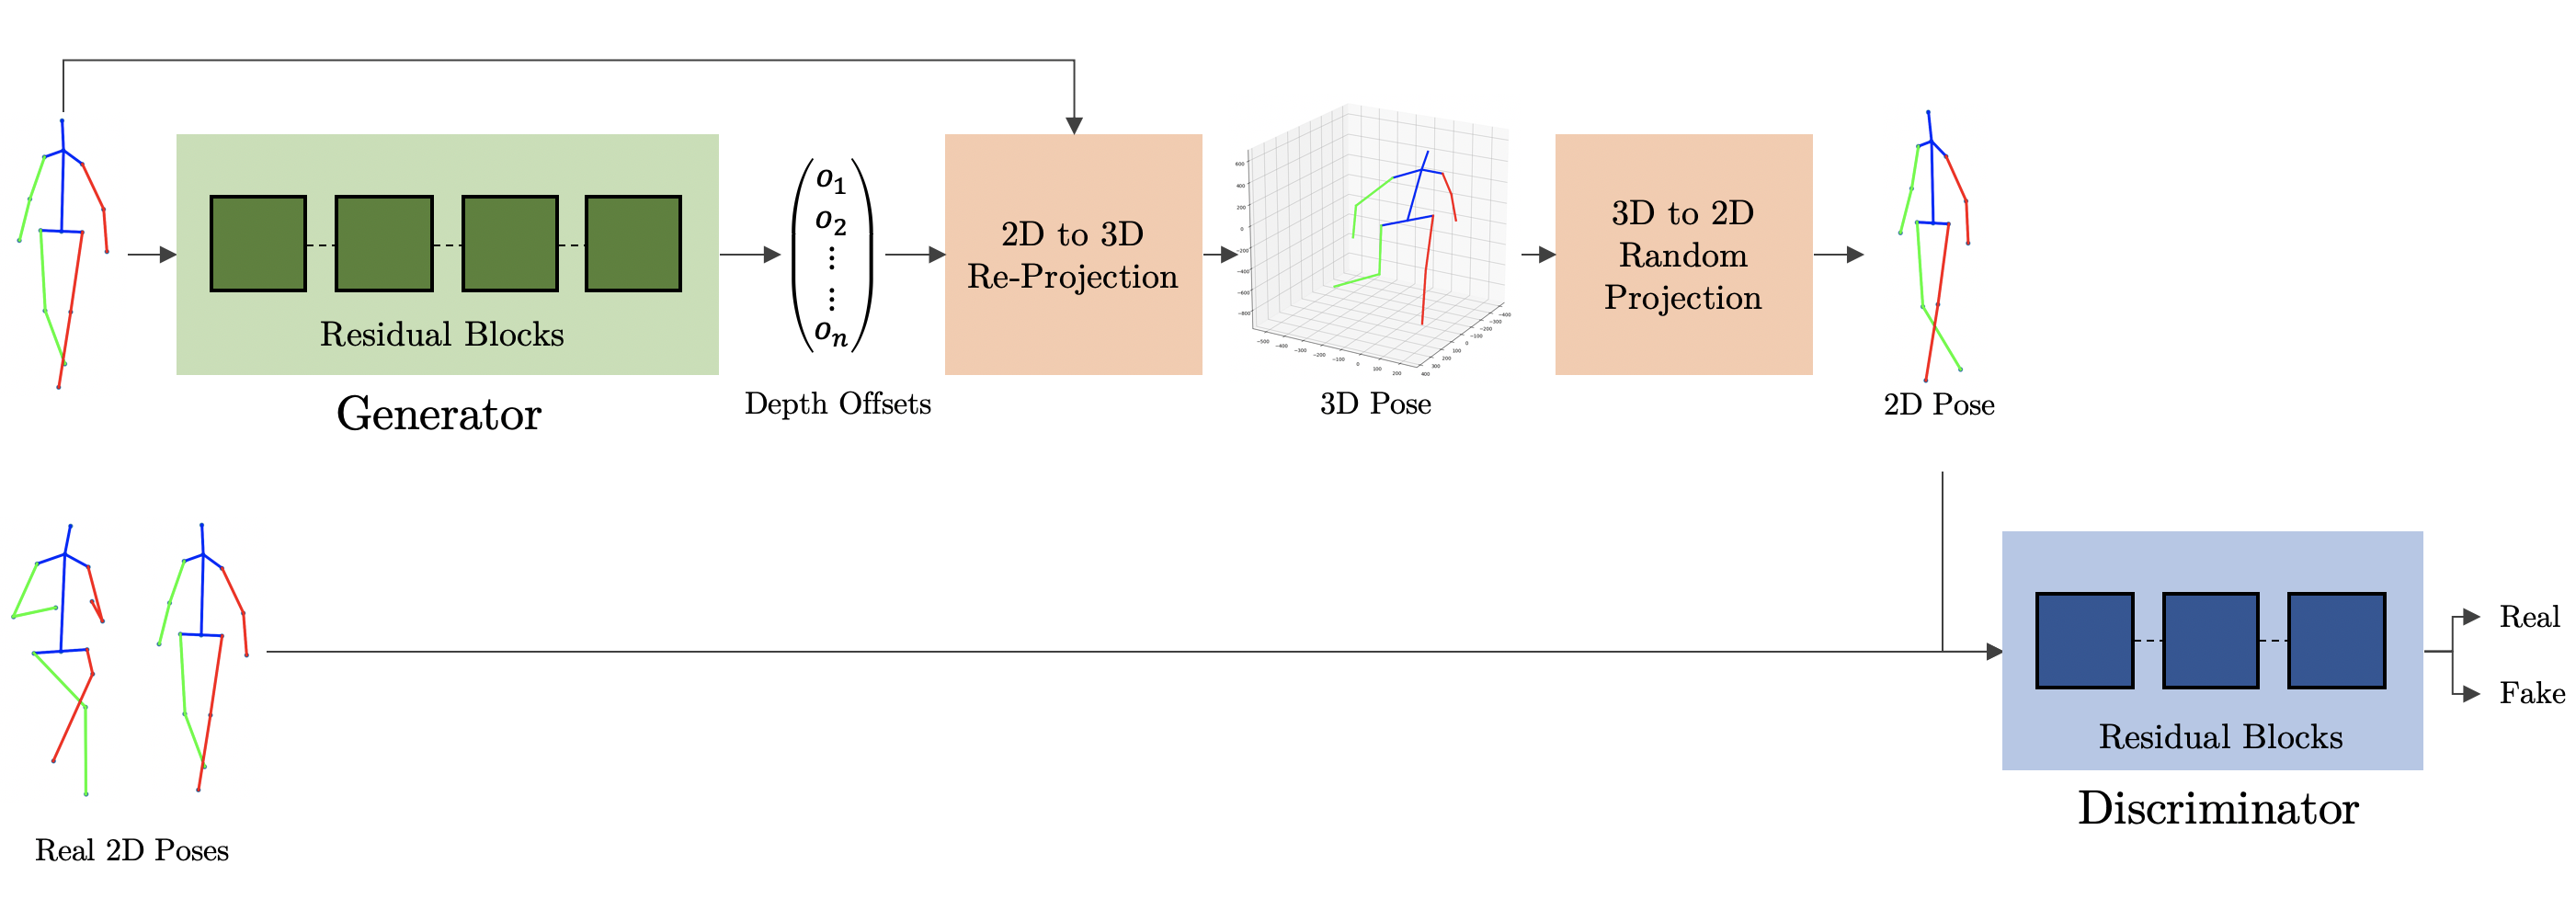
\includegraphics[width=1.1\textwidth]{figures/system.png}
	}
	\caption{The core of this thesis: The 2D to 3D pose GAN proposed by \citet{drover18}.}
	\label{fig:system}
\end{figure}

In their work, \citet{drover18} make use of a GAN in the context of 3D human pose estimation.
\autoref{fig:system} displays a diagram of their proposed system.
It follows the basic GAN architecture and adds some extra layers after the generator.
The architecture will be described in the following.

The generator's and discriminator's input are human 2D poses.
In practice, the generator's input pose is the pose to be lifted to 3D.
For numerical stability, \citet{drover18} require the input poses for both discriminator and generator to be normalized in the following way:
\begin{enumerate}[label=(\Alph*)]
	\item The 2D poses' root joint is centered at the origin of the image plane.
	\item A designated norm limb has length $0.1$.
\end{enumerate}
In this work, the root joint always is the pelvis (the center point between the hips) and the norm limb the connection (or distance) between pelvis and thorax.

In the system, the latent and the real distribution $p_z$ and $p_real$ are both the distribution of real 2D poses.
This means that the generator is also trying to learn that distribution.
On the way to doing that, 3D human poses are created as a byproduct, which can then be used in other applications.

In the proposed system, the generator receives 2D poses as input.
For those poses, it estimates the depth of each joint.
In order to eliminate the additional degree of freedom introduced by the scale-distance ambiguity (a 3D pose $P$ and a 3D pose $P'$ twice as far away from the camera and twice as big both project to the same 2D pose), the system aims to estimate 3D poses that have a norm limb length of $1$.
Hence, instead of an absolute depth, only a \emph{depth offset} $o_i$ is estimated for each joint $(x_i, y_i)$.
The absolute depths can then be calculated as
\begin{equation}
	\label{eq:depth-clipping}
	Z_i = \max \{f, Z + o_i\} \ .
\end{equation}
The clipping ensures that, at the time of re-projection, the points are projected in front of the camera.

Using the so found depths for each joint, the 2D pose can be re-projected into three dimensions using \autoref{eq:perspective-re-projection}.
In practice, the $Z$ in \autoref{eq:depth-clipping} is $10$, such that the re-projected poses have an approximate norm limb length of $1$.

Afterwards, the obtained 3D poses are fed into a \emph{Random Projection Layer}, where they are projected into two dimensions again.
For this, the poses are randomly rotated with with azimuth angles between $0$ and $360$ degrees and elevation angles between $0$ and $20$ degrees, first and then projected as in \autoref{eq:perspective-projection}.
Subsequently, those 2D poses are fed to the discriminator.

During training, the discriminator receives 2D poses from $p_{real}$ and $p_{fake}$ and tries to classify them as either real or fake, that is, as stemming from $p_{real}$ or $p_{fake}$.

\Todo{Find good way to typeset this.}
This system design is based on one underlying heuristic:\vspace{.5em}\newline
\vspace{.5em}
\noindent{\emph{If a random projection of a 2D pose looks realistic, the 3D pose is realistic.}}\newline
This heuristic is based on the fact that it is extremely unlikely for a malformed 3D pose to result in a realistic 2D pose when photographed from a random point of view.

\begin{figure}
	\centering
	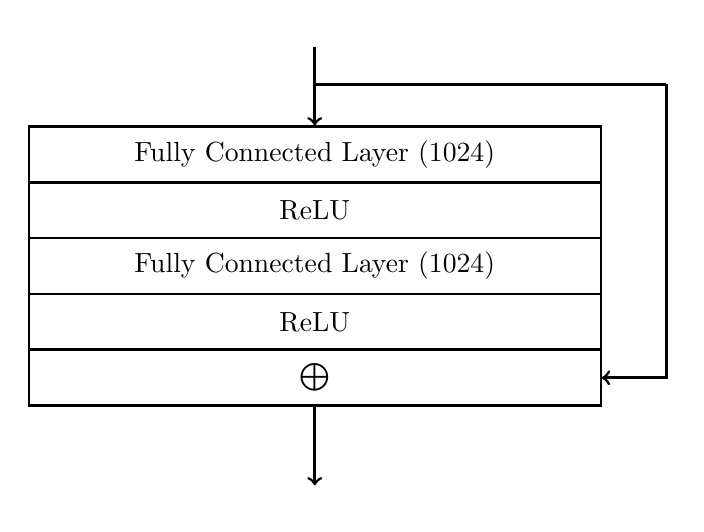
\begin{tikzpicture}
	[
	 block/.style ={rectangle, draw=black, thick, text width=20em, align=center, minimum height=2em}
	]
	\node[] (a) [block] {Fully Connected Layer (1024)};
	\node[below= -1.5\pgflinewidth of a] (b) [block] {ReLU};
	\node[below= -1.5\pgflinewidth of b] (c) [block] {Fully Connected Layer (1024)};
	\node[below= -1.5\pgflinewidth of c] (d) [block] {ReLU};
	\node[below= -1.5\pgflinewidth of d] (e) [block] {$\bigoplus$};
	\node[above=of a] (x) [] {};
	\draw[->, line width=1pt] (x) -- (a);
	\node[below=of e] (y) [] {};
	\draw[->, line width=1pt] (e) -- (y);
	\node[above=.4 of a] (z) [] {};
	\node[right=12em of z] (h) [] {};
	\draw[line width=1pt] (z.center) -- (h.center);
	\draw[->, line width=1pt] (h.center) |- (e.east);
	\end{tikzpicture}
	\caption{Architecture of the Residual Blocks in generator and discriminator.
	Two fully connected layers of size 1024 are each followed by a Rectified Linear Unit (ReLU). After the last ReLU the input is added to the output.
	\citet{drover18} suggest a Batch Normalization immediately after each Fully Connected Layer, which has not been found to work.}
	\label{fig:residual-block}
\end{figure}

In practice, both generator and discriminator are neural networks that consist of several consecutive \textit{Residual Blocks}.
A Residual Block consists of two fully connected layers of size $1024$ each followed by ReLU activation and a residual connection adding the input to the last layer's output (\autoref{fig:residual-block}).
In their work, \citet{drover18} describe two additional Batch Normalization layers \cite{ioffe15}, one immediately after each fully connected layer.
Practical tests have shown that when using those additional layers the training does not converge at all.
\unsure{Should I still mention the "personal communication"? I'm not sure if their paper is related to this work enough.}
As competitive results could also be achieved with the reduced network design, the proposed Batch Normalization Layers have been left out completely in this work.

Architecture-wise, the generator takes $n$ 2D joint locations (i.e. $2n$ scalar inputs) as input and feeds them to a fully connected layer of size 1024.
This is followed by four Residual Blocks and concluded by another fully connected layer of size 1024 mapping the output of the last residual block to a vector of size $n$, in which each entry represents the depth offset one joint.

The discriminator's architecture is very similar to the generator's. 
It also accepts $n$ 2D joint locations as input which are fed into a fully connected layer of size 1024, followed by three residual blocks.
The output is then reduced by another fully connected layer to a vector of size 2.
Finally, softmax is applied.
The resulting values imply the probability of the input being real or fake.

The networks are trained with the standard GAN losses described in Equations~\ref{eq:generator-loss} and~\ref{eq:discriminator-loss}.
	
	\section{Data}
\label{sec:data}

\begin{itemize}
	\item Common 3D datasets with 3D annotation. Very few annotated
	\item Motivation for training with 2D data only
	\item Different representations of poses (absolute points, angles, ...)?
\end{itemize}
 

For training and evaluation of the models the dataset Human3.6M \cite{ionescu14} is used. 
It contains 3.6 million three dimensional human poses captured by digital and motion capture cameras, consisting of data from 11 subjects (6 male, 5 female) performing 15 different activities such as walking, taking a photo, eating or smoking.
The poses are available in different parametrizations, but only the one with 3D joint positions transformed with the camera parameters of the 4 digital cameras were used for training and evaluation (called \texttt{D3\_Positions\_mono} in the dataset).
The dataset also contains the 2D projections of the monocular 3D poses onto the cameras' image plane.

\todo[inline]{32 joints and 15 / 17 joints; Pose = set of 3D joint locations}

In the literature multiple different evaluation methods are used. 
This is partly because not all models produce absolute 3D poses, but some only up to a scaling factor or alignment of joints.
Therefore, some modifications have to be made in order to measure the quality and allow a fair comparison to other approaches.
Essentially two different evaluation protocols with minor variations have emerged which will be presented and discussed in the following.

\subsection{Evaluation Metrics}
The most commonly used metric for evaluation is the \textit{Mean per Joint Position Error} (MPJPE).
For a pose with $n$ joints, original 3D joint positions $O_i$ and predicted positions $P_i$ it is defined as
\begin{equation}
	\frac{1}{n} \sum_{i = 1}^{n}  \norm{O_i - P_i}_2 \ .
\end{equation}


\Todo[inline]{Angle error}
\subsection{Protocol 1}

This protocol is used under different names in slightly different variations in \cite{sun17, drover18, moreno-noguer16, yasin16, kostrikov14, tome17}.
The method commonly referred to as \textbf{Protocol 1} uses subjects S1, S5, S6, S7, S8 and S9 for training and S11 for testing.

Sometimes the train data is thinned out further by the elimination of similar poses \cite{yasin16}.
\citet{drover18} even completely leave out S8 for training.
It allows rigid alignment \cite{drover18, yasin16, kostrikov14, sun17, tome17, chen17} of the predicted poses to the ground truth data.


Most authors do not explicitly state which kind of rigid alignment is applied to the predicted poses.
Those who do mention a Procrustes Analysis \cite{sun17, tome17} or a Least Squares transformation \cite{kostrikov14}.
That basically allows kinds of translation, scaling and rotation can be applied in order to best fit the predicted poses to the ground truth data.

This approach is not very realistic though as in production there is no ground truth data the predicted poses can be fitted to.
A more realistic testing technique is presented in the Section \ref{sec:protocol2}.

In accordance with the code shipped with the Human3.6M dataset, \citet{sun17}, \citet{chen17} and \citet{moreno-noguer16} use only every \nth{64} frame of the available data for testing.



%
\section{Protocols}
\subsection{Protocol 1}
	\begin{itemize}
		\item Training: S1, S5, S6, S7, S8, S9 (commonly used, e.g. in \cite{chen17})
		\begin{itemize}
			\item \cite{drover18} do not use S9.
			\item The available code suggests that not every pose is used, but only such where at least one joint has moved by 40mm with respect to the former frame.
		\end{itemize} 			
		\item Evaluation: S11
		\begin{itemize}
			\item \cite{sun17} use every 64th frame (and also the code suggests this). If they only use the available code this would mean they use all four cameras.
			\item \cite{drover18} use ground truth 2d points for testing (might be the same as \cite{sun17})
			\item \cite{moreno-noguer16} use every 64th frame of the frontal view for testing
		\end{itemize}

		\item Error: \begin{itemize}
			\item \cite{drover18} use Mean per Joint Position Error (MPJPE) with scaling and rigid alignment to the ground truth skeleton (they don't mention which exactly)
			\item \cite{sun17} also use MPJPE after rigid alignment using Procrustes Analysis
			\item \cite{yasin16} use the MPJPE after alignment to the ground truth skeleton by a rigid transformation (they don't mention which exactly)
			\item \cite{kostrikov14} align the poses by a rigid transformation using \emph{least squares} before computing the MPJPE error
			\item \cite{tome17} perform a similarity transformation using a Procrustes Analysis
		\end{itemize}
		
	\end{itemize}
\subsection{Protocol 2}
	\begin{itemize}
		\item Training: S1, S5, S6, S7, S8
		\begin{itemize}
			\item Similar to protocol 1 the code suggests that not every pose is used, but only such where at least one joint has moved by 40mm with respect to the former frame.
			\item \cite{bogo16} evaluate on five different action sequences captured from the frontal camera
			\item \cite{tekin16, tekin17} use all camera views for training
		\end{itemize}
		\item Evaluation: S9, S11 
		\begin{itemize}
			\item \cite{sun17} use every 64th frame
			\item \cite{tekin16, tekin17} use all camera views for testing
			\item \cite{bogo16} evaluate on five different action sequences captured from the frontal camera
			\item \cite{moreno-noguer16} say they use all images for testing (whatever this means) 
		\end{itemize}
		\item Error: \begin{itemize}
			\item \cite{sun17} use MPJPE apparently without any alignment and scaling
			\item \cite{martinez17} align the root (central hip), they do not mention any scaling
			\item \cite{tome17} do not mention any alignment
			\item \cite{zhou18} scale the output such that the mean limb length is identical to the average value of all training subjects and align the root locations. Procrustes Analysis is not allowed.
			\item \cite{bogo16} apply a similarity transformation to align the reconstructed 3D joints via the Procrustes analysis on every frame
			\item \cite{zhou16} align the root locations and scale the output such that the mean limb length is identical to the average value of all training subjects. Procrustes alignment is not allowed.
			\item it seems that \cite{tekin16} also align the root nodes
			\item \cite{tekin17} use a Procrustes transformation before measuring the MPJPE
			\item \cite{pavlakos17} align the root joints
		\end{itemize}
	\end{itemize}

\subsection{Miscellaneous}
\begin{itemize}
	\item \cite{jahangiri17} evaluate using all subjects after a similarity transformation obtained by Procrustes alignment
\end{itemize}

\section{Questions and Problems}
\begin{itemize}
	\item It is sometimes not clear which 2d poses are used for testing.
	\item The transformations applied before calculating the error are not consistent within the protocols.
\end{itemize}


\section{Our approach}
	\subsection{Protocol 1}
		\begin{itemize}
			\item Training subjects: S1, S5, S6, S7, S8, S9
			\item Testing/Evaluation subjects: S11
			\item For now we train on all frames available, \emph{not} such where at least one joint has moved by 40mm
			\item For evaluation every 64th frame available for the according subjects is used
			\item Error metric: MPJPE
			\item Before calculating the error, the poses are transformed using a Procrustes Transformation and the root nodes are aligned
		\end{itemize}
	\subsection{Protocol 2}
		\begin{itemize}
			\item Training subjects: S1, S5, S6, S7, S8
			\item Testing/Evaluation subjects: S9, S11
			\item For now we train on all frames available, \emph{not} such where at least one joint has moved by 40mm
			\item For evaluation every 64th frame available for the according subjects is used
			\item Error metric: MPJPE
			\item Before calculating the error, the root nodes are aligned and the pose is scaled such that the mean limb length is identical to the average value of all training subjects
		\end{itemize}

\begin{itemize}
	\item Dataset Human3.6m
	\item Original and augmented data
	\item Data used for training, evaluation and testing.
\end{itemize}
\subsection{Protocol 2}\label{sec:protocol2}

The second protocol found in the literature is \textbf{Protocol 2}.
In this case only S1, S5, S6, S7 and S8 are used for training, while test results are reported for S9 and S11.

Whereas \citet{sun17} only use every \nth{64} frame and \citet{moreno-noguer16} and \citet{bogo16} only use camera 3 for testing, most authors do not mention which poses exactly are used for testing.

This protocol only allows certain noninvasive changes to the predicted poses.
In general rigid alignment like a Procrustes Analysis is not allowed.
The degree of the changes applied to the predicted poses strongly depends on the model.
In a system that predicts absolute 3D poses usually no changes have to be made to the predicted poses in order to obtain meaningful results.
With only a monocular 2D projection of a pose, it is not possible to estimate the absolute 3D poses as there are multiple 3D poses which all have the same 2D projection.
Therefore many models \cite{martinez17, zhou18, zhou16, tekin16, pavlakos17} allow aligning two designated root joints (usually the central hip) of the predicted and the ground truth poses.
In cases where it is not possible to correctly estimate the global scale of the poses scaling is also allowed.
\citet{zhou18} do this by scaling the predicted poses such that "the mean limb length is identical to the average value of all training subjects".
This is still suboptimal because if the subjects have different mean limb lengths (which is the case) the error for a perfect prediction would not be 0.
A better way of scaling would be the following:

First, calculate the average limb length $L_s$ of all poses for each subject $s$.
Then, scale each predicted and ground truth pose in a way that the mean limb length is equal to $L_s$.

Because adjusting the ground truth data is not a good practice in general, in this thesis only the predicted poses are scaled to match $L_s$.

\subsection{Training data}\label{sec:data-results}

Unfortunately the 2D poses included in the dataset are not suitable for training the network supposed by \citet{drover18}, as both assumptions (1) and (2) are not satisfied.
Hence - similar to the work of \citet{drover18} - synthetic 2D data is generated by randomly projecting the monocular 3D poses.
First, the poses are normalized the same way as in Section \ref{sec:network} and then photographed by cameras with integer azimuth and elevation angles randomly sampled from $[0, 359]$ and $[0, 19]$ and a distance of 10 units.
Finally, the obtained 2D poses are normalized again.


\begin{itemize}
	\item Results for self created data
	\item Results for original 2d data
\end{itemize}

	\section{Baseline Results for Synthetic and Real Data}
\label{sec:evaluation}

Later in this work, the effects of pose normalization in the system by \citet{drover18} will be analyzed, both theoretically and experimentally.
In a first step towards the experimental analysis, baseline results for a rebuilt version of the system have to be established.
Those results provide insights about the system's performance under different conditions and ease a comparison between the original system by \citet{drover18} and modified versions of this system which will be presented in later sections.

\subsection{Training Procedure and Hyperparameters}
For training, the Adam Optimizer \cite{kingma17} with an initial learning rate of $2 \cdot 10^{-4}$ and $\beta_1 = 0.5$ is used for both generator and discriminator.
This particular choice of $\beta_1$ has shown to result in faster convergence.
As in the work by \citet{drover18}, the data is split up into batches of $32768$ poses.
Generator and discriminator are trained alternately with the same batch of poses, for up to $50000$ iterations until convergence.
Before adjusting the networks' parameters, adaptive clipping is applied to the gradients \cite[Section~3.2.1]{chorowski14}.


\subsection{Results for Training with Synthetic Data}

The 2D input poses of the system are required to fulfill the constraints (A) and (B) from \autoref{sec:network-architecture}. 
They state that the poses' root joint has to be centered at the origin of the image plane and that the poses are required to have a norm limb length of $0.1$, that is, be normalized in location and scale.
For an input pose to match those constraints there are two options:
\begin{enumerate}
	\item The input pose already naturally fulfills the constrains by being projected with certain extrinsic camera parameters.
	\item The input pose does not fulfill the constraints and has to be transformed with translation and scaling.
\end{enumerate}
In order to analyze the effects of the normalization in the second case, poses not fulfilling the constraints have to be compared to poses that already naturally satisfy them.
Thus, a baseline for (1) has to be established.
For this, the 2D poses included in the Human3.6M are not viable because the cameras used to project the 3D poses do not have the special extrinsic parameters required.
Informally, those parameters can be described as follows:
The camera has to be centered at the root joint in order to fulfill (A). 
Furthermore the camera distance to the 3D pose has to be such that the projected norm limb has a length of 0.1 (fulfilling constraint (B)).

Hence, synthetic 2D poses are generated by projecting the 3D poses included in Human3.6M with those extrinsic parameters.
For training and testing, cameras centered at the root joint with integer azimuth and elevation angles randomly sampled from $[0, 359]$ degrees and $[0, 20]$ degrees are used.
This choice of elevation angles is based on the heuristic that in reality, people are rather photographed from above than from below and also on the fact that the cameras in Human3.6M have similar angles.
For projection, the 3D poses are first normalized such that the norm limb has length 1 and then photographed with a camera-root-joint distance of $10$ units and a focal length of $1$.
With the specific choice of elevation angles, the projected root limb has a length usually close to 0.1 and only slight scaling is necessary.
For training, \citet{drover18} follow a similar procedure and augment synthetic 2D poses, although they use 8 fixed cameras instead of randomly sampled camera angles for each pose.

\begin{table}[]	
	\centering
	\begin{tabularx}{\textwidth}{l *{8}{Y}}
		\toprule
		Method & Direct. & Discuss & Eat & Greet & Phone & Pose & Purchase & Sit \\
		\midrule
		\citet{drover18} & 34.3 & 36.4 & 28.4 & 33.7 & 30.0 & 43.8 & 31.7 & 32.5\\
		Synthetic & 36.3 & 35.5 & 35.6 & 42.6 & 34.8 & 44.1 & 45.2 & 36.3 \\
		Human3.6M & 35.7 & 34.2 & 37.9 & 40.3 & 37.3 & 38.6 & 43.5 & 40.4 \\
		\bottomrule
		\toprule
		Method & SitDown & Smoke & TPhoto & Wait & Walk & WDog & WTog. & \textbf{Avg.}\\
		\midrule
		\citet{drover18} & 48.9 & 32.1 & 43.8 & 36.0 & 25.1 & 34.1 & 30.3 & \textbf{34.2}\\
		Synthetic & 51.9 & 41.9 & 50.8 & 43.0 & 38.5 & 49.6 & 40.8 & \textbf{41.0} \\
		Human3.6M & 59.7 & 45.0 & 52.6 & 42.2 & 32.5 & 45.8 & 36.0 & \textbf{41.2} \\
		\bottomrule
	\end{tabularx}
	\caption{
		Comparison of the MPJPEs reported by \citet{drover18} and for a rebuilt system trained with synthetic data. 
		The rebuilt system is tested with synthetic data ("Synthetic") and 2D poses from Human3.6M  \cite{ionescu14} ("Human3.6M").
		The results were obtained using \textbf{Protocol 1}. The MPJPEs are given in millimeters.
	 }
	\label{tbl:results-original-protocol1}
	\info[inline]{Augmented obtained with best.ckpt-16161 from e\_03\_07\_original.json;
		Human3.6M obtained with real 2D poses with best.ckpt-16161 from e\_03\_07\_original.json}
\end{table}
\begin{table}[]	
	\centering
	\begin{tabularx}{\textwidth}{l *{8}{Y}}
		\toprule
		Method & Direct. & Discuss & Eat & Greet & Phone & Pose & Purchase & Sit \\
		\midrule
		Synthetic & 48.8 & 51.5 & 41.5 & 57.7 & 49.4 & 54.3 & 48.8 & 50.0 \\
		Human3.6M & 86.5 & 81.7 & 65.2 & 86.6 & 82.4 & 85.2 & 93.6 & 61.3 \\
		\bottomrule
		\toprule
		Method & SitDown & Smoke & TPhoto & Wait & Walk & WDog & WTog. & \textbf{Avg.}\\
		\midrule
		Synthetic & 64.3 & 51.9 & 64.6 & 57.1 & 54.3 & 57.9 & 53.2 & \textbf{54.8} \\
		Human3.6M & 82.3 & 73.8 & 93.2 & 85.6 & 78.3 & 80.9 & 82.1 & \textbf{80.4} \\
		\bottomrule
	\end{tabularx}
	\caption{
		Comparison of the MPJPEs of the replicated system trained and tested with synthetic data and 2D poses from the Human3.6M dataset \cite{ionescu14}. 
		For \cite{drover18} only results with rigid alignment are available, which allows no fair comparison.
		The results were obtained using \textbf{Protocol 2}. The MPJPEs are given in millimeters.
	 }
	\label{tbl:results-original-protocol2}
	\info[inline]{Synthetic obtained with best.ckpt-16161 from e\_03\_07\_original.json;
	Human3.6M obtained with real 2D poses with best.ckpt-16161 from e\_03\_07\_original}
\end{table}
\begin{table}	
	\centering
	\begin{tabularx}{\textwidth}{l *{4}{Y}}
		\toprule
		Method & Acting3 & Freestyle3 & Walking2 & \textbf{Average}\\
		\midrule
		Protocol 1 & 65.5 & 74.7 & 65.7 & \textbf{68.3} \\
		Protocol 2 & 98.8 & 105.8 &  96.8 & \textbf{100.2} \\
		\bottomrule
	\end{tabularx}
	\caption{
		MPJPEs for the test data of the \textbf{TotalCapture} dataset \cite{trumble17}. The system was trained with synthetic data from Human3.6M.
		The results were obtained using the transformations of Protocol 1 and 2 as indicated. The MPJPEs are given in millimeters.
	 }
	\label{tbl:results-original-totalcapture}
	\info[inline]{Protocol 1 obtained with best.ckpt-16161 from e\_03\_07\_original.json;
	Protocol 2 obtained with best.ckpt-16161 from e\_03\_07\_original.json}
\end{table}

Table \ref{tbl:results-original-protocol1} shows the results for \textbf{Protocol 1} reported in \cite{drover18} and for the replicated system trained with the synthetic 2D poses.
For the evaluation of the latter, one synthetic 2D pose is deterministically sampled from each monocular 3D pose available for Subject 11 in the same way as before.
The results for the synthetic training data can not compete with the results presented by \citet{drover18}.
The exact source of the 6.8mm average discrepancy is not clear; there can be various reasons for it.
Those include the following:
\citet{drover18} don't mention whether they also use synthetic poses for testing or evaluate only on 2D poses provided in Human3.6M.
Another reason can be that before calculating the MPJPE, they apply a similarity transformation, but don't explicitly mention the Procrustes Analysis used in this work.
Further discrepancy can also arise from different internal configurations, such as the exact training procedure or the applied gradient clipping.
\citet{drover18} also report the use of Batch Normalization Layers in each of the residual blocks, which could not be found to work during the replication of their proposed system.
Finally, extensive mining for the best performing model might also be a reason for the lower MPJPE.

The results for \textbf{Protocol 2} are given in Table \ref{tbl:results-original-protocol2}.
They are not directly comparable to those by \citet{drover18} because the authors also allow rigid alignment (which includes rotation) for Protocol 2.
In this work, similar to most other literature, rotation is not allowed to fit the estimated poses to the ground truth for this protocol.
This is also the reason for the MPJPEs being approximately 14mm higher than those for Protocol 1.

Tables \ref{tbl:results-original-protocol1} and \ref{tbl:results-original-protocol2} also display evaluation results for the monocular 2D poses available in the Human3.6M dataset.
For Protocol 1, the MPJPEs for the different categories are approximately as good as those for the synthetic data, for some activities even better.
In contrast to this, the results for Protocol 2 are clearly worse than those for the synthetic data.
Here the error margin is at 25.6mm.
The key difference between Protocols 1 and 2 is that Protocol 1 permits rotation to fit the poses, as both protocols allow translation and scaling.
Hence, disregarding the absolute rotation of the poses, the results for the Human3.6M poses are overall just as good as those for the synthetic data.
Although this looks good from a theoretical point of view, for real world applications this is only helpful when the absolute rotation of the poses is not of interest.
Otherwise only the results for Protocol 2 are meaningful.

The system is also evaluated for a different dataset.
On the test data of TotalCapture \cite{trumble17}, the average MPJPE for Protocol 1 is 68.3mm and for Protocol 2 100.2mm respectively (Table \ref{tbl:results-original-totalcapture}).
The pose structure in this dataset is slightly different from Human3.6M, which could explain the higher error.
The most noticeable difference is the angle between the two hips.
In Human3.6M, this angle measures 180 degrees and the spine is perpendicular to the hips, whereas in TotalCapture the angle is substantially smaller (see Figure \ref{fig:human-totalcapture}).
Although the results for TotalCapture are slightly worse, they still show that the system generalizes to unseen data in a reasonable way.

\begin{figure}
	\centering
	\begin{minipage}{.45\textwidth}
		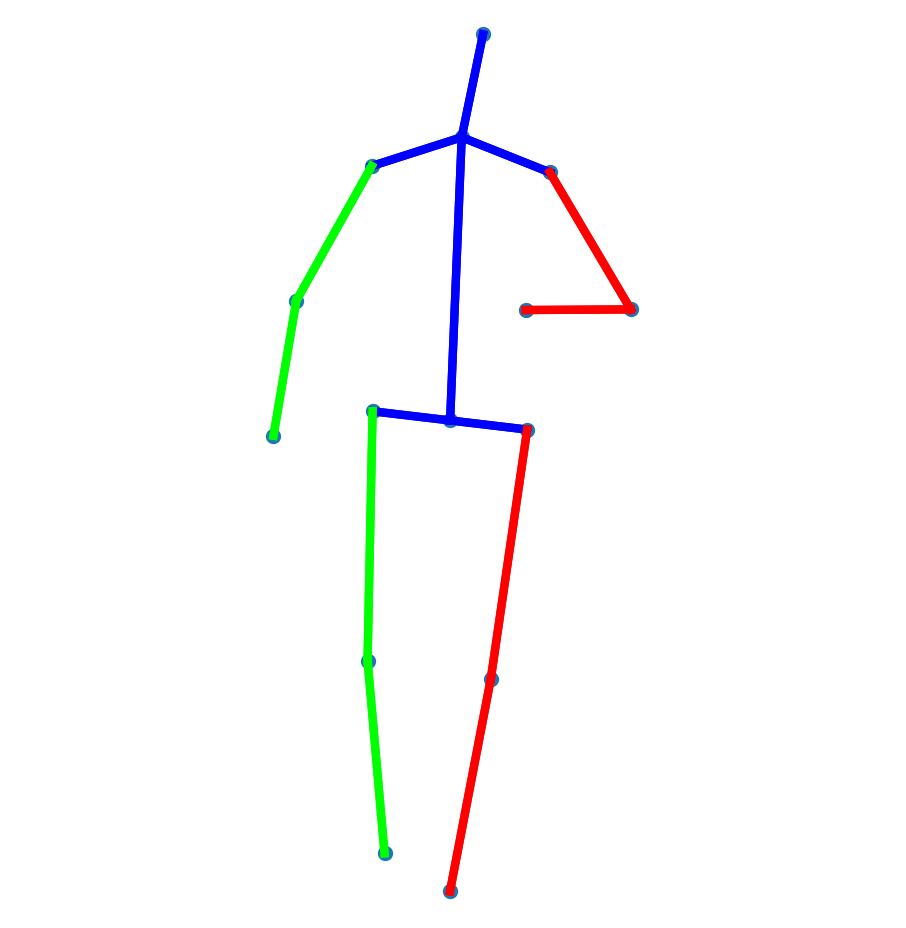
\includegraphics[width=.45\textwidth]{figures/2D_pose_human36m_1701.png}
		\scalebox{-1}[1]{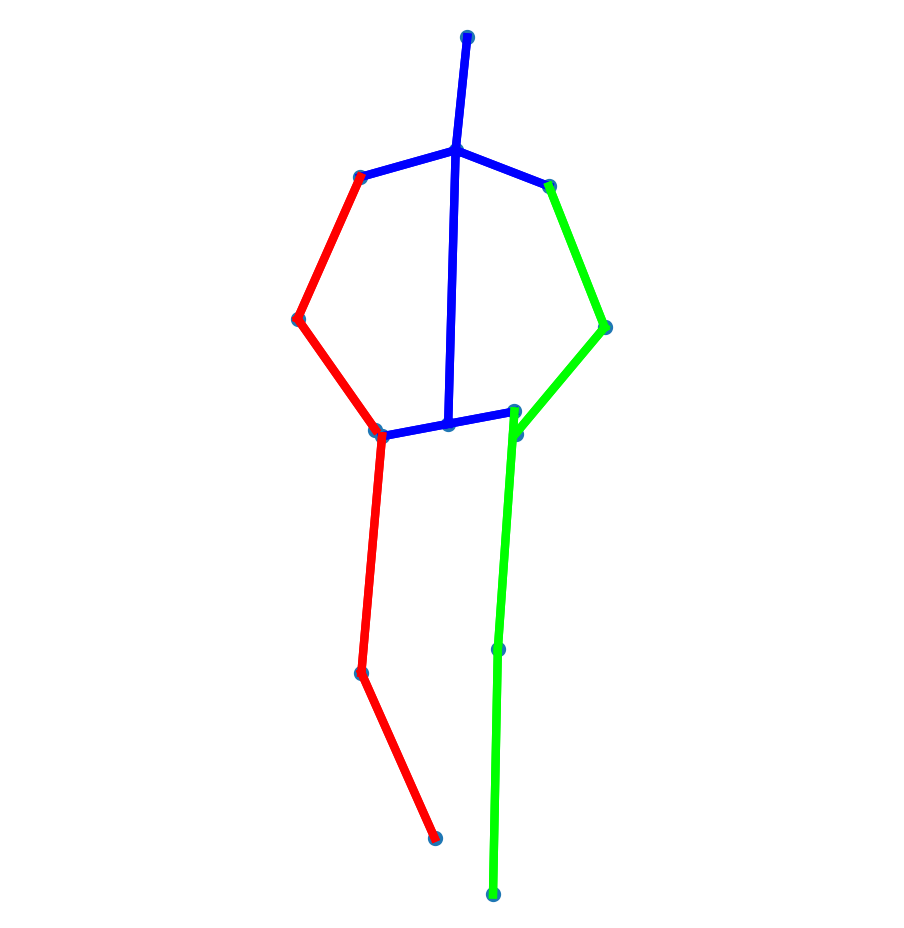
\includegraphics[width=.45\textwidth]{figures/2D_pose_human36m_4280.png}}
	\end{minipage}
	\hspace{5mm}
	\begin{minipage}{.45\textwidth}
	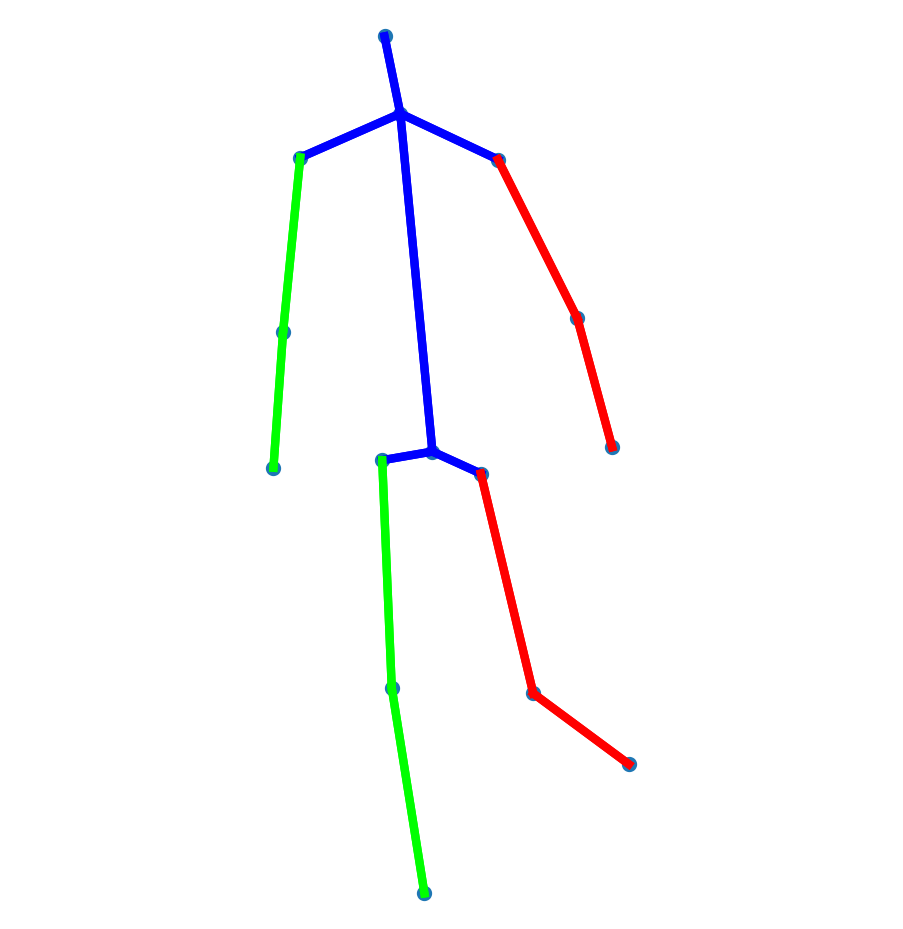
\includegraphics[width=.45\textwidth]{figures/2D_pose_totalcapture_24437.png}
	\scalebox{-1}[1]{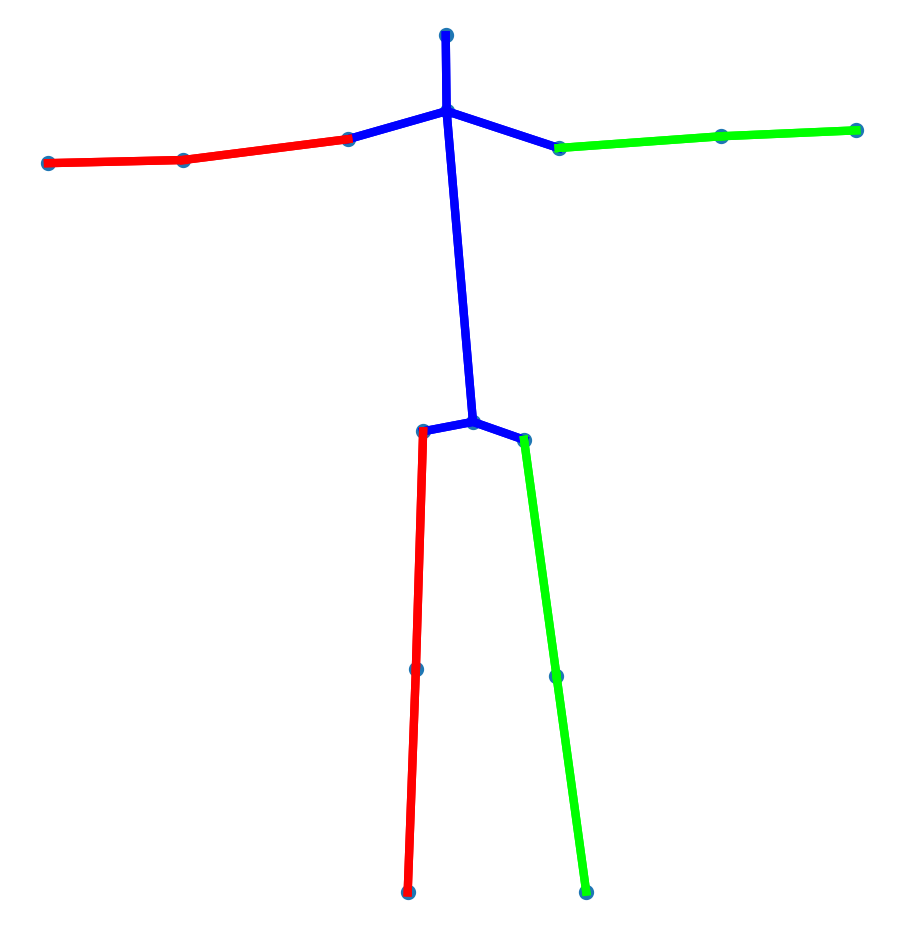
\includegraphics[width=.45\textwidth]{figures/2D_pose_totalcapture_102156.png}}
	\end{minipage}
	\caption{Comparison of two poses from the Human3.6M dataset (left) and two poses from the TotalCapture dataset (right).}
	\label{fig:human-totalcapture}
\end{figure}


\subsection{Results for Training with Augmented and Real Data}
\label{sec:results-augmented}
The results for the test data of the Human3.6M dataset are not quite satisfying, as they are only useful when rotation plays no role.
The reasons for the worse results may be of different nature:
A simple explanation is that machine learning systems tend to perform better on data which is more similar to the training data.
For the synthetic testing data this is certainly the case.
On the other hand, the results for Protocol 1 show that the poses are already sensible and only seem to lack the right orientation.
Another reason might be that Human3.6M's monocular 2D poses are in fact being normalized, both in scale and position, other than the synthetic data, which is already naturally normalized in position (and also almost in scale).

\Todo{Maybe try out training where the discriminator and the generator both receive the same dataset at 1:1 ratio, and augmented cameras}
In order to figure out whether the first conjecture contributes to the discrepancy, the monocular 2D poses are added to the training set.
A lower MPJPE would indicate that it does.
For training, the generator receives both real and synthetic poses at a 1:1 ratio.
As described in Section \ref{sec:network}, during training the generator tries to learn the real data distribution.
In order to have a chance to achieve this, it must be able to generate poses similar to the real poses. 
This comes down to the Random Projection Layer, where the poses are projected with a camera distance of $10$ and a root joint offset of $0$ (which means the camera is centered at the root joint).
2D poses projected with a camera distance other than $10$ or with a non-zero root joint offset are inherently different.
This will further be elaborated on in Section \ref{sec:effects-of-normalization}.
Thus there are two options:
Projecting the generated 3D poses with a camera distance and offset similar to the real data or feeding only data to the discriminator that resembles the generator's output.
As the real camera distance might not be known in general, and offsets would still need to be sampled, the second option is chosen.
This means the discriminator still only receives synthetic poses for training.

\begin{table}[]	
	\centering
	\begin{tabularx}{\textwidth}{l *{8}{Y}}
		\toprule
		Method & Direct. & Discuss & Eat & Greet & Phone & Pose & Purchase & Sit \\
		\midrule
		Synthetic & 48.8 & 51.5 & 41.5 & 57.7 & 49.4 & 54.3 & 48.8 & 50.0 \\
		Human3.6M & 48.8 & 51.5 & 41.5 & 57.7 & 49.4 & 54.3 & 48.8 & 50.0 \\
		\bottomrule
		\toprule
		Method & SitDown & Smoke & TPhoto & Wait & Walk & WDog & WTog. & \textbf{Avg.}\\
		\midrule
		Synthetic & 64.3 & 51.9 & 64.6 & 57.1 & 54.3 & 57.9 & 53.2 & \textbf{54.8} \\
		Human3.6M & 48.8 & 51.5 & 41.5 & 57.7 & 49.4 & 54.3 & 48.8 & 50.0 \\
		\bottomrule
	\end{tabularx}
	\caption{
		Comparison of the MPJPEs of the replicated system trained with monocular 2D poses from the Human3.6M dataset and synthetic data at a 1:1 ratio.
		The results are given for synthetic data and 2D poses from the Human3.6M dataset \cite{ionescu14}.
		The results were obtained using \textbf{Protocol 2}. The MPJPEs are given in millimeters.
	 }
	\label{tbl:results-real-and-synthetic-protocol2}
	\info[inline]{}
\end{table}

Table \ref{tbl:results-real-and-synthetic-protocol2} shows the results for both synthetic data and the monocular 2D test poses from Human3.6M for this data configuration.
While the results for the synthetic data are approximately the same as the ones in the previous section, the results for the Human3.6M poses improved by almost 8mm to 72.5mm.

A training with augmented cameras similar to the four real cameras available in Human3.6M showed no major improvement to this number.
For this, eight additional camera positions with equidistant azimuth angles were sampled.
Synthetic 2D poses were projected like above.
The Protocol 2 MPJPE for this setup is at 71.8mm.

These results have both positive and negative ramifications:
On the one hand, when the system is trained with real world data from a specific application, it will perform better in that application, compared to a pre-trained model.
On the other hand, this shows that the system is not able to generalize to all kinds of human poses with the same quality. 

\unsure[inline]{Should I use present, past or past progressive tense?
Should I also add (more) interpretation to the results (like e.g. to the error numbers)?}

	
	\section{\unsure{Too complex?}
	Exploiting Bilateral Symmetry for Improved Results}


In a standard fully-supervised network, training is heavily dependent on ground truth data.
As the key feature of the system described in this work is that only 2D poses are required for training, there is substantially lesser information available to the system during the training process.

In GANs, the generator only receives information about the distribution to be learned through the discriminator's error.
The discriminator on its part only receives information about the elements of the real data distribution.
Other than that, there is a priori no other information the generator can use to produce improved results.
Without ground truth data available, one of the only parts of additional knowledge that can be passed to the system during training are general, high-level facts that hold true for all elements of the distribution to be learned.

In the special case of human 3D pose estimation, such facts can be the kinematics or the basic structure of the human skeleton.
Generally, the movement of limbs relative to each other is highly constrained:
A leg can not (and if, only rarely) completely fold behind one's back and an hand cannot touch its own forearm.
If such information can be made available to the generator the results might improve.
However, everything exceeding simple restrictions for the relative angles between the limbs is highly complex and would be out of the scope of this work.
As the results from the previous section show that the generated poses already have sensible limb angles, it is not to be expected to gain any benefit by engineering knowledge about such simple kinematics into the system.

That leaves the basic structure of the human skeleton.
As all mammals, humans have a bilaterally symmetrical skeleton.
That symmetry can be made use of in the following way:
3D poses are expected to have equally long upper and lower arms, upper and lower legs, foots of equal size etc.
Also, the distance between the shoulders and the neck, and the hips and the base of the spine should not differ too much.
Concerning the GAN, that means this additional piece of information can be passed to the generator through the loss function.

Let a \emph{limb} $l = (u, v)$ be the connecting body part between joints $u$ and $v$.
For a set of symmetric limbs $S = \{(l_{i_1}, l_{i_2})~|~ l_{i_1}, l_{i_2}\ \text{are symmetric limbs} \}$ the \emph{limb loss} is defined as:
\begin{equation}
loss_{limb} = \frac{1}{|S|}\sum_{((u_1, v_1), (u_2, v_2)) \in S} \bigl\lvert \norm{u_1 - v_1}_2 - \norm{u_2 - v_2}_2 \bigr\rvert \ .
\end{equation}

The limb loss penalizes the generator if it produces poses with symmetric limbs of different lengths.
The new loss for the generator is then given by
\begin{equation}
	loss_{G, limb} = loss_G + \lambda \cdot loss_{limb} \ ,
\end{equation}
where $\lambda$ is a weighting factor and $loss_G$ is given in Equation \eqref{eq:generator-loss}.

\begin{figure}[bt]	
	\centering
	\begin{tabularx}{\textwidth}{l *{8}{Y}}
		\toprule
		Method & Direct. & Discuss & Eat & Greet & Phone & Pose & Purchase & Sit \\
		\midrule
		$loss_G$ & 88.8 & 88.8 & 88.8 & 88.8 & 88.8 & 88.8 & 88.8 & 88.8\\
		$loss_{G, limb}$ & 88.8 & 88.8 & 88.8 & 88.8 & 88.8 & 88.8 & 88.8 & 88.8 \\
		\bottomrule
		\toprule
		Method & SitDown & Smoke & Photo & Wait & Walk & WDog & WTog. & \textbf{Avg.}\\
		\midrule
		$loss_G$ & 88.8 & 88.8 & 88.8 & 88.8 & 88.8 & 88.8 & 88.8 & \textbf{88.8} \\
		$loss_{G, limb}$ & 88.8 & 88.8 & 88.8 & 88.8 & 88.8 & 88.8 & 88.8 & \textbf{88.8} \\
		\bottomrule
	\end{tabularx}
	\caption{
		Comparison of the MPJPEs with standard and modified loss for the Human3.6M dataset. 
		The results were obtained using \textbf{Protocol 2}.
	 }
	\label{fig:results-limb-loss}
\end{figure}

During training, $\lambda$ was increased linearly.
Initially it was set to $5$ and then increased by $0.002$ each iteration, until $\lambda = 100$.
That way, in the beginning the higher weighted standard loss ensures that the generator produces sensible 3D poses, and in later iterations the limb loss helps refining those poses.
Table \ref{tbl:results-limb-loss} shows the results of that training procedure.
For the 15 joint model, the employed symmetric limbs are the upper arms, the lower arms, the upper legs, the lower legs, the hips (distance from left and right hip to the root joint) and the shoulders (distance from shoulders to thorax). 
The generator trained with the modified loss is able to outperform the generator with standard loss in all categories.
The average MPJPE is reduced by 4.1mm to 50.7mm, which equals an improvement of more than 7\%.
For the individual categories the error is reduced by up to 8mm.

In conclusion, the limb loss function for the generator is an improvement to the work of \citet{drover18}.
As it comes at no cost, it can be easily integrated in future system.



	
	\section{Analysis of the Effects of Pose Normalization}
\label{sec:effects-of-normalization}

The original model of the 3D pose estimation system by \citet{drover18}, which is described in Section \ref{sec:network}, requires the input pose to be normalized in the following way:
\begin{enumerate}[label=(\Alph*)]
	\item The 2D input pose's root joint is centered at the origin.
	\item A designated norm limb has length 0.1.
\end{enumerate}

In reality both assumptions are rarely satisfied from the start.
Thus \citet{drover18} normalize the input 2D poses by shifting and scaling before feeding them to the generator.
In this chapter we will see both theoretically and experimentally that this approach inevitably leads to additional errors being introduced to the system.

\Todo[inline]{Figure of camera projection}

In the following we will assume that the camera used for projection is located at the origin of the coordinate system and looks into positive z direction.
All poses are assumed to have z coordinates greater than camera's focal length $f$ in order to be projected in front of the camera.
The generator $G$ will be regarded as a black box that takes a normalized 2D pose as input and outputs the depths (the z coordinates) of the input points which then can be reprojected into three dimensional space like in Equation \eqref{eq:perspective-re-projection}.

\Todo[inline]{
For simplicity, the problem will only be regarded in two dimensions.
For three dimensions the y coordinates are to be inserted at the appropriate places.
}

\subsection{Shifting along one image plane axis}
\label{sec:x-shift-error}
First we will analyze assumption (A) by examining a 3D pose $P$ which is centered at the origin of the x-y-plane.
$P$ is then shifted by the vector $(dx, dy, 0)$ along the x-y-plane and projected into two dimensions.
After the 2D pose has been aligned with the image plane's origin, it is re-projected into three dimensions.
The resulting 3D pose $\widetilde{P}$ will then be compared to the original 3D pose $P$ in order to gain insights in the additional error made through normalization.

Let $P = [(X_1, Y_1, Z_1), \dotsc, (X_n, Y_n, Z_n)]$ be a 3D pose.
For simplicity we will assume that $dy = 0$, that is, the pose $P$ is only shifted along the x axis.

\subsubsection{Theoretical analysis}
\label{sec:x-shift-error-theoretical}
Let $P_i = (X_i, Y_i, Z_i) \in P$.
Then the coordinates of the projected point on the image plane are given by
\begin{equation}
	x_i = f \frac{X_i}{Z_i} \ ,\enspace y_i = f \frac{Y_i}{Z_i} \ .
\end{equation}
Now assume that $P_i$ is shifted by $dx$ along the x axis.
This results in a projected x coordinate of
\begin{equation}
	\label{eq:projected-x-y}
	x_i^\mathrm{S} = f \frac{X_i + dx}{Z_i} = f \frac{X_i}{Z_i} + f \frac{dx}{Z_i} = x_i + f \frac{dx}{Z_i}\ .
\end{equation}
The projected pose is then normalized by shifting all projected points such that the root node is located in the origin of the image plane. 
Let the shifted root node have coordinates $(dx, 0, Z)$.
Since $dy = 0$, each point is only shifted by $- f \frac{dx}{Z}$ along the x axis.
That means the x coordinate of the normalized point $\widetilde{x}_i$ is given by
\begin{equation}
	\widetilde{x}_i
	= x_i^\mathrm{S} - f \frac{dx}{Z}
	= x_i + f \frac{dx}{Z_i} - f \frac{dx}{Z}
	= x_i + f dx (\frac{1}{Z_i} - \frac{1}{Z}) \ , 
\end{equation}
while the y coordinate stays the same as in \eqref{eq:projected-x-y}.
After $G$ estimates the depth $\widetilde{Z}_i$, the 2D point is reprojected into three dimensions using standard perspective projection. The resulting coordinates are 
\begin{align}
	\label{eq:re-projected-X}
	\widetilde{X}_i &= \frac{\widetilde{x}_i}{f} \cdot \widetilde{Z}_i
	= X_i \frac{\widetilde{Z}_i}{Z_i} + dx (\frac{1}{Z_i} - \frac{1}{Z}) \widetilde{Z}_i
	= \widetilde{Z_i} \left( \frac{X_i}{Z_i} + dx \left( \frac{1}{Z_i} - \frac{1}{Z} \right) \right) \ , \\
	\label{eq:re-projected-Y}
	\widetilde{Y}_i &= \frac{y_i}{f} \cdot \widetilde{Z}_i = \frac{Y_i}{Z_i} \cdot \widetilde{Z}_i \ .
\end{align}
The Euclidean distance (the Joint Position Error (JPE)) of the reprojected point to the original point is given by
\begin{equation}
\label{eq:delta-d}
	\Delta d_i = \norm{ 
	\begin{pmatrix}
		\widetilde{X}_i - X_i \\
		\widetilde{Y}_i - Y_i \\
		\widetilde{Z}_i - Z_i
	\end{pmatrix}
	}_2
\end{equation}
With perfect estimation of $\widetilde{Z_i} = Z_i$, we have $\widetilde{Y}_i = Y_i$ and Equation \eqref{eq:delta-d} together with \eqref{eq:re-projected-X} describes a linear relationship between the offset $dx$ and the Joint Position Error $\Delta d_i$.
But since the generator's estimation of $\widetilde{Z_i}$ can vary for different offsets $dx$, the JPE can actually become smaller for other $\widetilde{Z_i} \neq Z_i$. 
In order to obtain a correct lower bound for the Joint Position Error, we have to calculate the $\widetilde{Z_i}$ for which $\Delta d_i$ is minimal.
So the function to be minimized is
\begin{align}
	\label{eq:minimum-distance}
	f(\widetilde{Z}_i) &= \left ( \widetilde{Z}_i \cdot \left( \frac{X_i}{Z_i} + dx \left( \frac{1}{Z_i} - \frac{1}{Z} \right) \right ) - X_i \right)^2 + \left ( \widetilde{Z_i} \cdot \frac{Y_i}{Z_i} - Y_i \right )^2 + \left ( \widetilde{Z}_i - Z_i \right ) ^2 \\
	&= \left ( \widetilde{Z}_i \cdot a - X_i \right)^2 + \left ( \widetilde{Z_i} \cdot b - Y_i \right )^2 + \left ( \widetilde{Z}_i - Z_i \right )^2 \ ,
\end{align}
where $a \coloneqq \left( \frac{X_i}{Z_i} + dx \left( \frac{1}{Z_i} - \frac{1}{Z} \right) \right )$ and $b \coloneqq \frac{Y_i}{Z_i}$ have been substituted for better readability.
In order to obtain the optimal value for $\widetilde{Z}_i$, $f$ is differentiated by $\widetilde{Z}_i$:
\begin{equation}
	\label{eq:derivative-minimum-distance}
	f'(\widetilde{Z}_i) = 2 \cdot \left ( \widetilde{Z}_i \left (a^2 + b^2 \right ) - a X_i - b Y_i + \widetilde{Z}_i - Z_i \right )
\end{equation}
Setting this equal to zero gives
\begin{align}
	0 &= f'(\widetilde{Z}_i^\ast) \\
	\Leftrightarrow \widetilde{Z}_i^\ast & = \frac{a X_i + b Y_i + Z_i}{1 + a^2 + b^2} \ .
	\label{eq:z_i-min}
\end{align}
It is easy to see that $\widetilde{Z}_i^\ast$ is a minimum and $f$'s only extremum.
With $\widetilde{Z}_i^\ast$ the optimal $\widetilde{X}_i^\ast$ and $\widetilde{Y}_i^\ast$ from Equation \eqref{eq:re-projected-X} and \eqref{eq:re-projected-Y} can now be calculated:
\begin{align}
	\label{eq:x_i-min}
	\widetilde{X}_i^\ast &= \widetilde{Z}_i^\ast \cdot a
	= \frac{a^2 X_i + a b Y_i +  a Z_i}{1 + a^2 + b^2} \ ,\\
	\label{eq:y_i-min}
	\widetilde{Y}_i^\ast &= \widetilde{Z}_i^\ast \cdot b
	= \frac{b^2 Y_i + a b X_i + b Z_i}{1 + a^2 + b^2} \ . 
\end{align}

Putting \eqref{eq:z_i-min}, \eqref{eq:x_i-min} and \eqref{eq:y_i-min} into \eqref{eq:delta-d} yields a total minimal error of 
\Todo{Make roots look nice}
\begin{align}
	\Delta d_i &= 
	\sqrt{\left (\widetilde{X}_i^\ast - X_i \right )^2 + \left (\widetilde{Y}_i^\ast - Y_i \right )^2 + \left (\widetilde{Z}_i^\ast - Z_i \right )^2}\\
	& = \sqrt{\frac{\left (a Y_i - b X_i \right )^2 + \left (a Z_i - X_i \right )^2 + \left (b Z_i - Y_i \right )^2}{1 + a^2 + b^2}} \\
	\label{eq:bzy-zero}
	&= \sqrt{\frac{\left (dx \cdot Y_i \cdot \left (\frac{1}{Z_i} - \frac{1}{Z} \right) \right)^2 + \left (a Z_i - X_i \right )^2}{1 + a^2 + b^2}}\\
	& = \sqrt{\frac{\left (dx \cdot Y_i \cdot \left (\frac{1}{Z_i} - \frac{1}{Z} \right ) \right)^2 + \left (dx \cdot Z_i \cdot \left (\frac{1}{Z_i} - \frac{1}{Z} \right ) \right)^2}{1 + a^2 + b^2}} \\
	& = \sqrt{\frac{dx^2 \cdot \left (\frac{1}{Z_i} - \frac{1}{Z} \right )^2 \cdot \left (Y_i^2 + Z_i^2 \right ) }{1 + a^2 + b^2}}\\
	\label{eq:minimum-delta-d}
	& = \abs{dx \left (\frac{1}{Z_i} - \frac{1}{Z} \right )} \sqrt{\frac{(Y_i^2 + Z_i^2)}{1 + a^2 + b^2}} \ .
\end{align}
In Equation \eqref{eq:bzy-zero} $b Z_i - Y_i = 0$ has been used.
With this $\Delta d_i$ the MPJPE for the whole pose can then be calculated as the mean of all $\Delta d_i$s:
\begin{equation}
	\label{eq:minimum-mpjpe-on-shift}
	\Delta d = \frac{1}{n} \sum_{i = 1}^{n} \Delta d_i 
\end{equation}
In contrast to the linear relationship for $\widetilde{Z_i} = Z_i$, for optimal $\widetilde{Z_i}$, the minimal MPJPE converges to a constant for large $dx$.

This result shows that even with the generator estimating the depth of each point optimally, the estimated 3D pose will never match the original 3D pose up to shifting and scaling.
Especially the re-projection of the 2D poses into three dimensional space without first shifting the 2D poses back as they were before normalization adds an essential part to the MPJPE.
In fact, the effects of 2D pose normalization by shifting only vanish if $dx = 0$ or $Z_i = Z$ for all $i$. 
In the latter case all joints of the pose are located in a plane parallel to the image plane.

The theoretical results above also show another downside of normalization by shifting.
In case the generator is trained with 2D poses which have multiple different offsets $dx$ and $dy$, ambiguities are introduced to the system:
As the generator can't know whether the pose it receives was originally located in the origin of the image plane or not, it can't correctly learn which depth offset belongs to which pose.
\unsure{Should possible solutions already presented here?}
One easy solution for this second problem is to train only with poses that all have the same offsets in x and y direction.
As this is rarely the case in reality, that would make the system only viable for very specific tasks in practice.

\unsure{Mention the intuition behind the phenomenon: Shift means we see the pose more from the side.}

\subsubsection{Experimental results}

Figure \ref{fig:x-shift-error} depicts a plot of the observable MPJPEs (measured using Protocol 2; Section \ref{sec:protocol2}) for 2D poses sampled from subjects 9 and 11 with different offsets in x direction along with a plot of the minimal MPJPE calculated in the previous section in Equation \eqref{eq:minimum-mpjpe-on-shift}.
As it turns out, both curves have the same approximate shape, but the sampled poses' MPJPE is significantly smaller than the theoretical MPJPE.
The difference between the two curves is increasing for larger offsets $\abs{dx}$.
At first glance, this seemingly contradicts the fact that the above $\Delta d$ represents a lower bound for the error.

One important detail has not been taken into account yet:
During the evaluation with Protocol 2, shifting and scaling might be applied to the estimated poses. 
For the root joint $r$ we have $Z_i = Z$ in \eqref{eq:minimum-delta-d}, so $\Delta d_r = 0$. That means $(\widetilde{X}_i, \widetilde{Y_i}, \widetilde{Z}_i) = (X_i, Y_i, Z_i)$, that is, the root nodes of both poses are already aligned.
It is not as easy to make a statement about scale of the pose $\widetilde{P}$ from a theoretical point of view only though.
Experimental results show that the average limb length of $\widetilde{P}$ is increasing monotonously with increasing offset $\abs{dx}$.
That means for a fair comparison with the observable results for Protocol 2 each pose $\widetilde{P}$ has to be re-scaled by a factor $\alpha_{\widetilde{P}}$ in all dimensions before the MPJPE is calculated:
\begin{equation}
	\Delta d_i = \norm{ 
	\begin{pmatrix}
		\alpha_{\widetilde{P}} \cdot \widetilde{X}_i - X_i \\
		\alpha_{\widetilde{P}} \cdot \widetilde{Y}_i - Y_i \\
		\alpha_{\widetilde{P}} \cdot \widetilde{Z}_i - Z_i
	\end{pmatrix}
	}_2 \ .
\end{equation}

\begin{figure}
	\begin{subfigure}[]{.3\textwidth}
		\centering
		\begin{tikzpicture}[trim axis left]
		\begin{axis}[
			tiny,
			width=1.25\textwidth,
			xlabel={$dx$ [m]},
%			axis lines = middle,
    		y label style={at={(axis description cs:0.35,1.15)},rotate=-90,anchor=north},
			ylabel={MPJPE [mm]},
			grid=both,
			enlarge x limits = false,
			grid style={draw=gray!50},
			minor tick num = 1,
			tick style={draw=gray!50},
			xtick={-100,-50,0,50,100},
			extra x ticks={0},
			scaled x ticks = false,
			no markers,
			every axis plot/.append style={}
		]
		\addplot table [x=a, y=b, col sep=comma] {figures/plot_e_03_07_original_x_shift.csv};
		\addplot table [x=a, y=b, col sep=comma] {figures/plot_theoretical_x_shift.csv};
		\end{axis}
		\end{tikzpicture}
		\subcaption{unscaled}
	\end{subfigure}\hfill
	\begin{subfigure}[]{.3\textwidth}
		\centering
		\begin{tikzpicture}[trim axis left]
		\begin{axis}[
						tiny,
			width=1.25\textwidth,
			xlabel={$dx$ [m]},
			%			axis lines = middle,
			y label style={at={(axis description cs:0.35,1.15)},rotate=-90,anchor=north},
			ylabel={MPJPE [mm]},
			grid=both,
			enlarge x limits = false,
			grid style={draw=gray!50},
			minor tick num = 1,
			tick style={draw=gray!50},
			xtick={-100,-50,0,50,100},
			extra x ticks={0},
			scaled x ticks = false,
			no markers,
			every axis plot/.append style={}
		]
		\addplot table [x=a, y=b, col sep=comma] {figures/plot_e_03_07_original_x_shift.csv};
		\addplot table [x=a, y=b, col sep=comma] {figures/plot_theoretical_x_shift_scaled.csv};
		\end{axis}
		\end{tikzpicture}
		\subcaption{scaled}
	\end{subfigure}\hfill
	\begin{subfigure}[]{.3\textwidth}
		\centering
		\begin{tikzpicture}[trim axis left]
			\begin{axis}[
				tiny,
				width=1.25\textwidth,
				xlabel={$dx$ [m]},
				%			axis lines = middle,
				y label style={at={(axis description cs:0.35,1.15)},rotate=-90,anchor=north},
				ylabel={MPJPE [mm]},
				grid=both,
				enlarge x limits = false,
				grid style={draw=gray!50},
				minor tick num = 1,
				tick style={draw=gray!50},
				xtick={-3,-2,-1,0,1,2,3},
				extra x ticks={0},
				scaled x ticks = false,
				no markers,
				every axis plot/.append style={}
				]
				\addplot +[restrict expr to domain={\coordindex}{180:401}] table [x=a, y=b, col sep=comma] {figures/plot_e_03_07_original_x_shift.csv};
				\addplot +[restrict expr to domain={\coordindex}{180:401}] table [x=a, y=b, col sep=comma] {figures/plot_theoretical_x_shift_scaled.csv};
			\end{axis}
		\end{tikzpicture}
		\subcaption{scaled}
	\end{subfigure}
			

	
	\caption{Theoretical (red) and experimental (blue) MPJPEs for different values of $dx$.
		The original theoretical minimal MPJPE does not represent a lower bound (a), meanwhile the one with scaled joint coordinates does (b and c). 
		The theoretical errors are obtained by calculating $\Delta d$ for every pose in the Protocol 2 test data.
		The distance between the camera and the poses is approximately 5m.}
	\label{fig:x-shift-error}
	\unsure[inline]{Should the plots be larger? Are angles better than absolute offsets as the x axis?}
\end{figure}
 
A plot of the resulting function for the minimal error is shown in Figure \ref{fig:x-shift-error}.
Here is is clearly visible that Equation \eqref{eq:delta-d} represents a lower bound to the MPJPE.

It is also noticeable that the performance of the network is not worse than the theoretical results by a constant offset.
For small deviations along the x axis the network seems to be able to compensate the error introduced by shifting.
As $dx$ increases, so does the offset between the observed and the theoretical results until it seems to converge to a constant.

As shown in Section \ref{sec:evaluation} the MPJPE for the monocular 2D poses of the Human3.6M dataset is about 25mm higher than the one for the synthetically generated data.
As those poses' root joints mostly have non-zero x and y offsets, the phenomenon discussed above might contribute to the error.


The simplest explanation for this is that the original 2D poses do not fulfill the constraints for the system.
The camera is not centered on the root joint and also the camera distance is most certainly not exactly ten times the length of the norm limb.

Numbers: ...
	
\subsection{Shifting along the z axis}
\label{sec:z-shift-error}

In this section, assumption (B) will be analyzed.
It states that a 2D pose's designated norm limb should have length $0.1$ when the pose is fed to the generator.
In case the assumption is not fulfilled from the start, there can be two reasons for this: 
An incorrect focal length $f$ of the camera, or an either to large or to small distance $Z$ between the camera and the 3D pose's root node.

In case $Z$ is fixed for all poses and only the focal length of the camera is incorrect, the pose can be normalized without any problems.
As the focal length is only a scale factor the projected points are multiplied with, dividing by it results in the same 2D pose as if $f$ has been correct in the first place.

But when the focal length $f$ of the camera is fixed and the incorrect length of the norm limb is caused by the distance between the camera and the root node, normalization by scaling will introduce an additional error.
The intuitional explanation behind this is that the projection rays' relative angles change when the 3D pose is projected with greater or smaller distance.
The resulting MPJPE will be analyzed in the following section.

\subsubsection{Theoretical analysis}
Again consider a point $P_i=(X_i, Y_i, Z_i) \in P$ and a camera with focal length $f$. Assume that $P_i$ is shifted by $dz$ along the z axis.
The x coordinate of the projected point on the image plane is
\begin{equation}
	x_i = f \frac{X_i}{Z_i + dz}
\end{equation}
The projected points are now scaled such that they have the same (arbitrary) scale, that is, a norm limb length of 0.1.
Let $\alpha$ be the scale factor of the original projected points and $\beta$ be the one of the shifted projected points. 
The x coordinate of the scaled projected point is given by
\begin{equation}
		\widetilde{x}_i = x_i \cdot \frac{\alpha}{\beta} 
		= f \frac{X_i}{Z_i + dz}\cdot \frac{\alpha}{\beta} 
\end{equation}
After the generator estimates the depth $\widetilde{Z}_i$, the point is re-projected into three dimensional space.
The re-projected point is given by
\begin{equation}
	\widetilde{X}_i = \frac{\widetilde{x}_i}{f} \cdot \widetilde{Z}_i
	= \frac{X_i}{Z_i + dz}\cdot \frac{\alpha}{\beta}  \cdot \widetilde{Z}_i
\end{equation}
Like in Section \ref{sec:x-shift-error-theoretical}, the Euclidean distance to the original point should be minimized with respect to $\widetilde{Z_i}$.
We consider the function
\begin{equation}
	f(\widetilde{Z}_i) = \left ( \widetilde{Z}_i \cdot \frac{X_i}{Z_i + dz}\cdot \frac{\alpha}{\beta} - X_i \right)^2 + ( \widetilde{Z}_i - Z_i )^2 \ .
\end{equation}
If we define $a \coloneqq \frac{X_i}{Z_i + dz}\cdot \frac{\alpha}{\beta}$, we can obtain the same derivative as in Equation \eqref{eq:derivative-minimum-distance}.
So with the same optimal 
\begin{equation}
	\widetilde{Z_i} = \frac{a X_i + Z_i}{1 + a^2} \ ,
\end{equation}
we can obtain a total minimal JPE of 
\begin{equation}
	\label{eq:z-shift-error}
	\Delta d_i = \sqrt{\frac{(a Z_i - X_i)^2}{1 + a^2}} 
	= \abs{\frac{X_i dz}{Z_i + dz}} \sqrt{\frac{1}{1 + a^2}} \ .
\end{equation}
Again, the MPJPE $\Delta d$ of the whole pose $P$ can be calculated as the mean of all $\Delta d_i$s (Equation \eqref{eq:delta-d}).

In contrast to the results of the previous sections, this theoretical result is not as directly applicable to the system.
Before the evaluation with Protocol 2, the root nodes of the estimated and ground truth poses are aligned.
If the generator estimates the depths $\widetilde{Z}_i = Z_i + dz$ for all $i$, the estimated pose $\widetilde{P}$ equals $P$ up to a shift.


In general, there exists no factor $\gamma$ such that $x_i = \widetilde{x_i}$ for all $i$ (to be precise, such factor only exists if for all $i$ $Z_i = \widetilde{Z_i}$).
That means the shifted projected pose and the original projected pose usually do not match.
Thus, if the generator receives poses with different total depths, it can not know with which camera distance the pose has been captured.


\subsubsection{Experimental results}
\label{sec:error-on-shift-experimental}

This phenomenon is also affecting our ground truth data. The poses are all projected with a camera distance $ \text{length-of-norm-limb} \cdot 10$. 
That means the length of the projected norm limb is not exactly $0.1$ but a bit smaller or bigger. 
Like discussed above those projected poses are then normalized. 
The system estimates the depths of the normalized pose and re-projects it assuming a perfect perspective projection. 
It therefore does not consider the effect of small deviations in z direction.
A way to fix this would be to calculate the perfect camera distance for each pose individually before projecting them onto the image plane.
This is not very realistic though since one might be able to determine the camera's distance to a human approximately, but definitely not exactly. This phenomenon therefore is kind of inevitable.

It can be hoped that the generator can compensate for small deviations in $Z$ by itself.

	
	\section{Prevention of the Effects of Pose Normalization}
\label{sec:network-adjusting}

The results of the previous section show that the network proposed by \citet{drover18} is not viable for practical use as is.
Especially if the camera photographing the poses was not centered at the root joint, a significant increase in MPJPE is measurable.
This motivates further looking into how this increased error can be circumvented.
This section will focus on the error introduced by shifting along the image plane, to be precise on shifting along the x axis, as it shows more significant additional MPJPE than shifting along the z axis.

In Equation \eqref{eq:re-projected-X}, if the point would be re-projected correctly (i.e. shifted back before re-projection), the theoretical lower bound would no longer hold true.
In that case, if the generator estimates all depths perfectly the re-projected pose equals the ground truth pose up to a shift.
Thus, in a first attempt to efface the error, the re-projection of the poses into three dimensional space will be adapted.

\subsection{Correct Re-Projection}

For a correct re-projection of the 2D poses into three dimensions, the network presented earlier is slightly modified.
The network now receives poses that are only normalized in scale, but not in location.
In a first step, the vector $(dx, dy)^\mathrm{T}$ given by the root joint's coordinates is subtracted from all 2D points, such that the 2D poses are now normalized both in scaled and in location.
Afterwards, the depth offsets $o_i$ are estimated for each point in the same way as in the original network.
Before the pose is then re-projected into three dimensions, the points are shifted back by adding $(dx, dy)^\mathrm{T}$ to each point again.

\begin{figure}
		\centering
		\begin{tikzpicture}[trim axis left]
		\begin{axis}[
		tiny,
		width=\textwidth,
		height=\axisdefaultheight,
		xlabel={$dx$ [m]},
		%			axis lines = middle,
		y label style={at={(axis description cs:0.13,1.1)},rotate=-90,anchor=north},
		ylabel={MPJPE [mm]},
		grid=both,
		enlarge x limits = false,
		grid style={draw=gray!50},
		minor tick num = 1,
		tick style={draw=gray!50},
		xtick={-10,-9,...,10},
		extra x ticks={0},
		scaled x ticks = false,
		no markers,
		every axis plot/.append style={}
		]
		\addplot +[restrict expr to domain={\coordindex}{90:491}] table [x=a, y=b, col sep=comma] {figures/plot_e_03_07_original_x_shift.csv};
		\addplot[color=black!60!green] table [x=a, y=b, col sep=comma] {figures/plot_e_01_06_shifted_generator_x_shift.csv};
		\addplot[color=red] table [x=a, y=b, col sep=comma] {figures/plot_e_11_08_default_generator_x_shift.csv};
		\addplot[color=orange] table [x=a, y=b, col sep=comma] {figures/plot_e_03_07_original_correct_reprojection_x_shift.csv};
		\end{axis}
		\end{tikzpicture}
	\caption{
		Comparison of MPJPEs for different networks. A pre-trained version of the original system with correct re-projection of the 2D poses (orange) outperforms the original system (blue).
		Training the former from ground up (red) reduces the MPJPE significantly, especially for larger offsets $dx$.
		If the generator with correct re-projection is trained with poses only normalized in scale, but not in location, the MPJPE decreases even more (green).
		The MPJPEs are calculated using Protocol 2.
		The distance between the camera and the poses is approximately 5m.}
	\label{fig:x-shift-error-correct-reproj}
	\Todo[inline]{Use correct data for shifted generator (data with cross entropy loss)}
\end{figure}

For the evaluation of this modified network, a pre-trained version of the original network in combination with the correct re-projection is utilized.
Protocol 2 MPJPEs are calculated for different offsets $dx$, while $dy = 0$.
The results for this procedure are shown in Figure \ref{fig:x-shift-error-correct-reproj}.
\Todo{Add evaluation once results are available.}

Comparison to modified network trained from scratch.
The 3D poses are normalized before the Random Projection Layer in order to avoid having to sample offsets.
The discriminator still only receives the normalized 2D input poses.


\subsection{Modified Network}
The correct re-projection of the 2D points into three dimensions without further adaption of the network was already able to reduce the MPJPE for shifted poses.
In an attempt to achieve the same MPJPE for all offsets $dx$, the network receives an additional piece of information.
On top of the correct re-projection, the vector $(dx, dy)^\mathrm{T}$ is now passed to the network alongside the 2D input pose.
In theory this should eliminate any ambiguities existing because of the normalization.

The network's input is now a vector of size $32$. 
The first $30$ elements are the coordinates of the normalized input pose's 15 joints, and the last two elements are the offsets $dx$ and $dy$.
During training the generator receives poses which have an offset $dx$ between $-10$m and $10$m.
As before, in order to avoid sampling offsets for the Random Projection Layer, the discriminator receives only such 2D poses which have an offset of $dx = 0$, while $dy = 0$.

Experimental results showed that\dots

New network tested with Human3.6M monocular 2D poses.

	
	\section{Conclusion}
\label{sec:conclusion}
In this thesis, the 2D to 3D human pose estimation system by \citet{drover18} has been analyzed with respect to the applied pose normalization.
In their work "Can 3D Pose Be Learned from 2D Projections Alone?", the authors propose a Generative Adversarial Network in which the generator estimates the depths for each of the 2D input pose's joints.
With those depths, a 3D pose can be obtained by re-projecting the 2D pose using the perspective projection equation.
The core feature of the system is that it can be trained solely using real 2D poses.
No 3D ground truth data is required.
For that, random projections of the estimated 3D poses are fed to the discriminator, which tries to distinguish between those and real 2D poses.

\autoref{sec:data} is about 3D human pose datasets, in particular the Human3.6M \cite{ionescu14} dataset.
The two evaluation protocols used in the context of this dataset were presented and discussed.
As the implementation of those protocols varies in literature, a noninvasive way of transforming the estimated poses was suggested for Protocol 2.
This transformation allows aligning two predefined root joints and scaling the poses to match the average limb length of the ground truth poses for each subject in the test dataset.
This comes close to the transformations that can be applied during application, and thus gives good insight about the quality of the poses in that scenario.

In \autoref{sec:evaluation}, a re-implemented version of the system has been evaluated for different data configurations.
The results reported by \citet{drover18} could only be reproduced up to a $6.8$mm margin when trained on synthetic 2D poses with an overall MPJPE of $41.0$mm for Protocol 1 (which allows rigid alignment through a Procrustes Transformation) and $54.8$mm for Protocol 2.
For the monocular 2D poses included in the Human3.6M dataset, the same results could only be achieved for Protocol 1; for Protocol 2 the MPJPE increased to $80.4$mm.
When trained with those poses in addition to the synthetic poses, the error could be reduced by about $10$mm.

In \autoref{sec:loss-function-modification} an improved loss function for the generator has been presented.
Humans have a pair-wise symmetrical skeleton with many limbs known to have equal lengths.
The suggested loss function punishes the generator if it produces symmetric limbs of different lengths, by adding the difference of two symmetric limbs to the standard GAN loss for the generator.
For training, the influence of the new term was increased over time.
With the new loss, the MPJPE could be reduced from $54.8$mm to $50.7$mm for Protocol 2; an improvement of more than $7\%$.

In \autoref{sec:effects-of-normalization}, the effects of pose normalization on the proposed system have been analyzed theoretically and experimentally.
The input poses are expected to be normalized in scale and location.
It has been shown that the normalization in location introduces a major error to the system, that increases for 2D poses having larger offsets from the camera's principal axis.
Experimental results confirmed the theoretical lower bound.
If the need for normalization in scale originates from a varying focal length of the camera, there is no error.
On the other hand, if the poses have to be re-scaled due to a varying camera distance, an additional error can be found.
As this error is relatively small, especially for small camera distance variations, it should be negligible in most applications.

In the last section, \autoref{sec:network-adjusting}, the system suggested by \citet{drover18} has been modified to compensate the effects of pose normalization through alignment.
When the generator receives poses that are only normalized in scale, but not in location, and re-projects those poses correctly into three dimensions, an almost constant performance for poses with varying offsets could be achieved.
For poses that are $10$m off the camera center (at a camera distance of $5$m), in the modified system the MPJPE only increases by about $15$mm, compared to the previous $285$mm.
	
	\newpage
	\Todo{Replace arxiv links with doi or link to journal where possible}
	\bibliography{bibliography}
	\bibliographystyle{plainnat}
	
\end{document}